\section{The failure-conditioned law in the critical window}\label{sec:window}
This section studies the regime in which the load is close to the peeling threshold and success and failure have comparable
probability. Section~\ref{sec:sign} has already handed the role of the sign composition to the factor $\gamma$; what remains is to
answer how the failure event selects the mapping in the all-same-sign case. Section~\ref{sec:score} introduces a precritical score
that predicts the success or failure of peeling. Section~\ref{sec:thm} states the main theorem: measurement and score are
asymptotically joint Gaussian, failure is asymptotically equivalent to the score being below zero, and the failure-conditioned law is
therefore the restriction of a bivariate normal to a half-plane. Section~\ref{sec:mean} reads off the conditional mean, variance, and
quantile from this truncated distribution, and Section~\ref{sec:flip} explains why the sign of the correlation coefficient changes
between $k=4$ and $k=5$.

\subsection{The peeling bottleneck and the precritical score}\label{sec:score}
Fix an integer $k\ge3$ and let $x_c$ be the unique positive root of $e^{x}-1=(k-1)x$.
The critical load is\cite{molloy,dn,jl07}
\begin{equation*}
\alpha_c=\frac{x_c}{k(1-e^{-x_c})^{k-1}}.
\end{equation*}
Closed forms for the remaining critical constants are collected in Appendix~\ref{app:constants}. Consider a deterministic sequence
\begin{equation}
\frac dM=\alpha_c+\frac r{\sqrt M}+o(M^{-1/2}),\qquad
r\in\mathbb R,\qquad\rho\longrightarrow\rho_\infty\in[-1,1].\label{eq:window}
\end{equation}
Here $r$ is fixed, and the limiting failure probability lies in $(0,1)$.

When the load is near the critical value, the peeling process passes through a bottleneck. Each step of peeling removes an edge
incident to a degree-one vertex and changes the degrees of the neighboring vertices, possibly creating new degree-one vertices or
destroying existing ones. When the load is slightly below $\alpha_c$, the density of degree-one vertices first drops close to zero and
then recovers; when the load is slightly above $\alpha_c$, the density drops below zero at its minimum and peeling halts. This minimum is
the bottleneck, and whether it can be crossed determines success or failure.

The precritical score $R$ reads the degree histogram before the bottleneck is reached and extrapolates how many degree-one vertices
remain at the bottleneck. Concretely, $R$ is a linear functional of the degree-one density of the corresponding profile at the
bottleneck, and its value depends only on the degree changes along the segment of the peeling path before the bottleneck is reached. A
negative remainder means that peeling will halt at the bottleneck. The window coordinate $r$ shifts the center of this remainder: for
$r<0$ the center is negative and the failure probability exceeds $1/2$; for $r>0$ the center is positive and the failure probability
is below $1/2$. The randomness of the mapping gives the remainder Gaussian fluctuations. The full construction of $R$ is in
Appendix~\ref{sec:mp-traj}; the main text only needs that it depends only on the unsigned mapping, is invariant under element-label
permutation, and its sign asymptotically determines the success or failure of peeling.

The correlation between measurement and score comes from the fluctuations of the cell degrees in the initial mapping. A mapping with
more overlap on the one hand changes the count energy (Section~\ref{sec:sign}), and on the other makes some cells have higher degree
and others lower degree, changing the degree profile and hence the remainder of peeling at the bottleneck. Both statistics are
functions of the initial degrees, and their correlation comes from this common source.

\subsection{Main theorem}\label{sec:thm}
\begin{theorem}[critical window joint limit]\label{thm:main}
Under the Plain model and the scaling~\eqref{eq:window}, there exists a precritical score $R$ that does not depend on the signs and is
invariant under element-label permutation. Let $\beta_k<0$, $\sigma_k>0$, and $a_c$ be the constants from
Appendix~\ref{app:constants}, and set
\begin{equation}
\eta_k=\frac{e^{-x_c}a_c(x_c-2)}{\sqrt{2\sigma_k^2}}.\label{eq:eta}
\end{equation}
\begin{enumerate}
\item[(i)] All-same-sign case:
\begin{align}
\left(X_{\rm one},\frac{R-\beta_k r}{\sigma_k}\right)
&\Rightarrow N\!\left(0,\begin{pmatrix}1&\eta_k\\\eta_k&1\end{pmatrix}\right),\label{eq:joint}\\
\Pr\bigl(F\triangle\{R\le0\}\bigr)&\longrightarrow0.\label{eq:transfer}
\end{align}
\item[(ii)] General sign composition: $(X,(R-\beta_kr)/\sigma_k)$ is asymptotically standard bivariate normal with correlation
$c=\eta_k\rho_\infty^2$.
\item[(iii)] Let $z_r=-\beta_k r/\sigma_k$. Then
\begin{gather*}
\Pr(F)\longrightarrow\Phi(z_r),\\
\sup_{x\in\mathbb R}\left|\Pr(X\le x\mid
F)-\frac{\Phi_2(x,z_r;c)}{\Phi(z_r)}\right|\longrightarrow0,
\end{gather*}
where $\Phi_2(\cdot,\cdot;c)$ is the standard bivariate normal distribution function with correlation $c$.
\end{enumerate}
\end{theorem}

The core of the theorem is (i), whose proof sketch is in Appendix~\ref{sec:proof-sketch} and full proof in
Appendix~\ref{sec:main-proof}. The correlation between measurement and score comes entirely from the initial mapping; the
fluctuations that the peeling process itself contributes to the score are asymptotically independent of measurement and only dilute the
correlation, so $|\eta_k|<1$. (ii) follows directly from (i) and Theorem~\ref{thm:sign}: $X=\gamma X_{\rm one}+V$, with $V$
asymptotically independent of $(X_{\rm one},R)$ and $\gamma\to\rho_\infty^2$, so the correlation between $X$ and the score is
$\eta_k\rho_\infty^2$. (iii) requires both \eqref{eq:joint} and \eqref{eq:transfer}. The former fixes the joint fluctuations of
measurement and score; the latter guarantees that the event that the score is below zero indeed describes the true peeling failure.
Together they give $\Pr(X\le x,F)\to\Phi_2(x,z_r;c)$, and dividing by the nonzero limiting failure probability yields the conditional
distribution. Since the limiting distribution is continuous, pointwise convergence can be lifted to uniform convergence of the
distribution functions.

Geometrically, the failure-conditioned law is obtained by restricting the limiting bivariate normal to the half-plane
$\{(x,y):y\le z_r\}$ and then looking at the first coordinate, where $y$ is the standardized score. For $c<0$, samples with low score
tend to have high measurement, and the selection shifts measurement to the right overall; for $c>0$ measurement shifts left overall;
for $c=0$ the selection has no effect. The smaller $z_r$ is, the farther the retained half-plane is from the center, the lower the
failure probability, and the more pronounced the shift. Figure~\ref{fig:joint} illustrates this truncation: (a) shows the limiting
density cut by the half-plane, and (b) gives a finite-size instance using the same batch of samples as Figure~\ref{fig:demo} in the
introduction. measurement and score are negatively correlated, the failing samples concentrate on the side where the score is below
zero, and their measurement is therefore high; this is the origin of the rightward shift of the failing samples in
Figure~\ref{fig:demo}(a).
\begin{figure}[!htbp]
\centering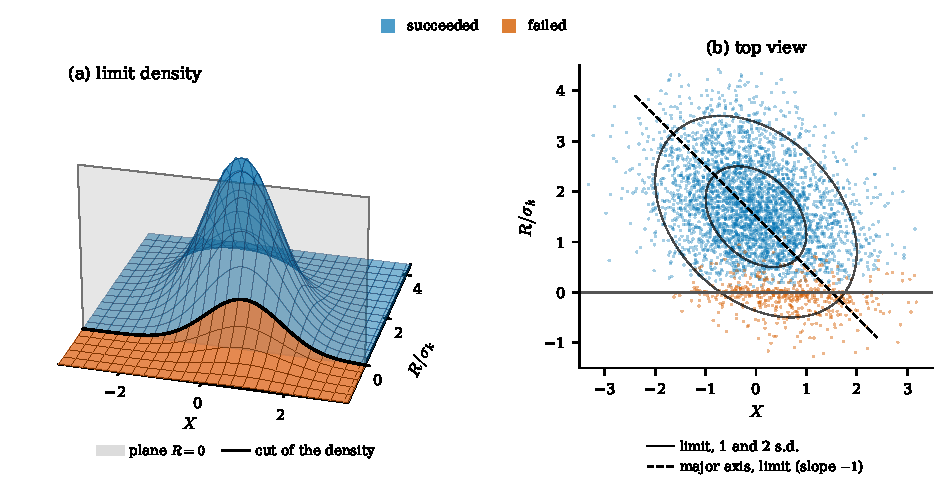
\includegraphics[width=\linewidth]{figures/fig-selection-joint.pdf}
\caption{Joint distribution of measurement and precritical score in the all-same-sign case ($k=3$, $M=16384$,
failure rate $0.125$). (a) Density of the limiting joint Gaussian; the gray plane is $R=0$, the orange part in front of the plane
corresponds to failure, and the black line is the cut;
(b) Top view in the same coordinates; each point is one Plain hypergraph, the ellipses are the one- and two-standard-deviation
contours of the limiting distribution, the dashed line is its major axis (slope $-1$), and the major axis of the sample covariance has
slope $-1.03$.}
\label{fig:joint}
\end{figure}
